\newpage
\section{SCD}
\thispagestyle{fancy}


\gls{SCD} utgjør grunnlaget for det meste av programmeringsdokumentasjonen i vår oppgåve.
Diagrammet er delt opp sidevis og sekvensvis og viser styring mellom program og komponentar i kvar enkelt sekvens
samt ei side for resterande felles styring.

Prosessen i \gls{SCD}en (i blå linjer) er basert på \gls{PID} som blei laga etter gjennomgangen av anlegget i kapittel 7.
\gls{SCD} tar kunn hensyn til programerbart utstyr og har derfor ikkje med manuelle ventilar, tilbakeslagsventilar og liknande utstyr.

Grunna valget rundt å bruke tilstandslogikk-blokker i programmet var vi nøydt å legge til våre eigne funksjonsblokker inn i diagrammet.
Dette hadde \gls{SCD} verktøyet ein funksjon for. \newline
Funksjonsblokkene våre og IEC funksjonstemplata i diagrammet er dei same blokkene som vi har laga og brukt i programmeringsdelen 
og dei stiplede linjene viser koplingar og styringa mellom dei. \newline
I enkelte av diagramma gjorde antall stiplede linjer diagrammet vanskeleg å lese. Vi har derfor benytta oss av koplingar med
unik ID for å illustrere tilknyttninga.

Heile \gls{SCD} er tilgjengelig i Appendix xXx
Våre tilstanslogikkblokker har fått eigne forkortingar i \gls{SCD}en. Desse er dei relevante forkortingane 
for å forstå blokkene og diagrammet.

\begin{itemize}
    \item \textbf{SM}:   State machine
    \item \textbf{FBP}:  Function Block Pause
    \item \textbf{FBI}:  Function Block Innpumping
    \item \textbf{FBR}:  Fucntion Block Reaksjon
    \item \textbf{FBS}:  Function Block Sedimentering
    \item \textbf{FBU}:  Function Block Uttapping
    \item \textbf{FBPH}: Function Block Pumpehus
\end{itemize}

\begin{tikzpicture}[remember picture, overlay]
    % Include the PDF page rotated, positioned at the center of the page
    \node[inner sep=0pt] at (current page.center) {
        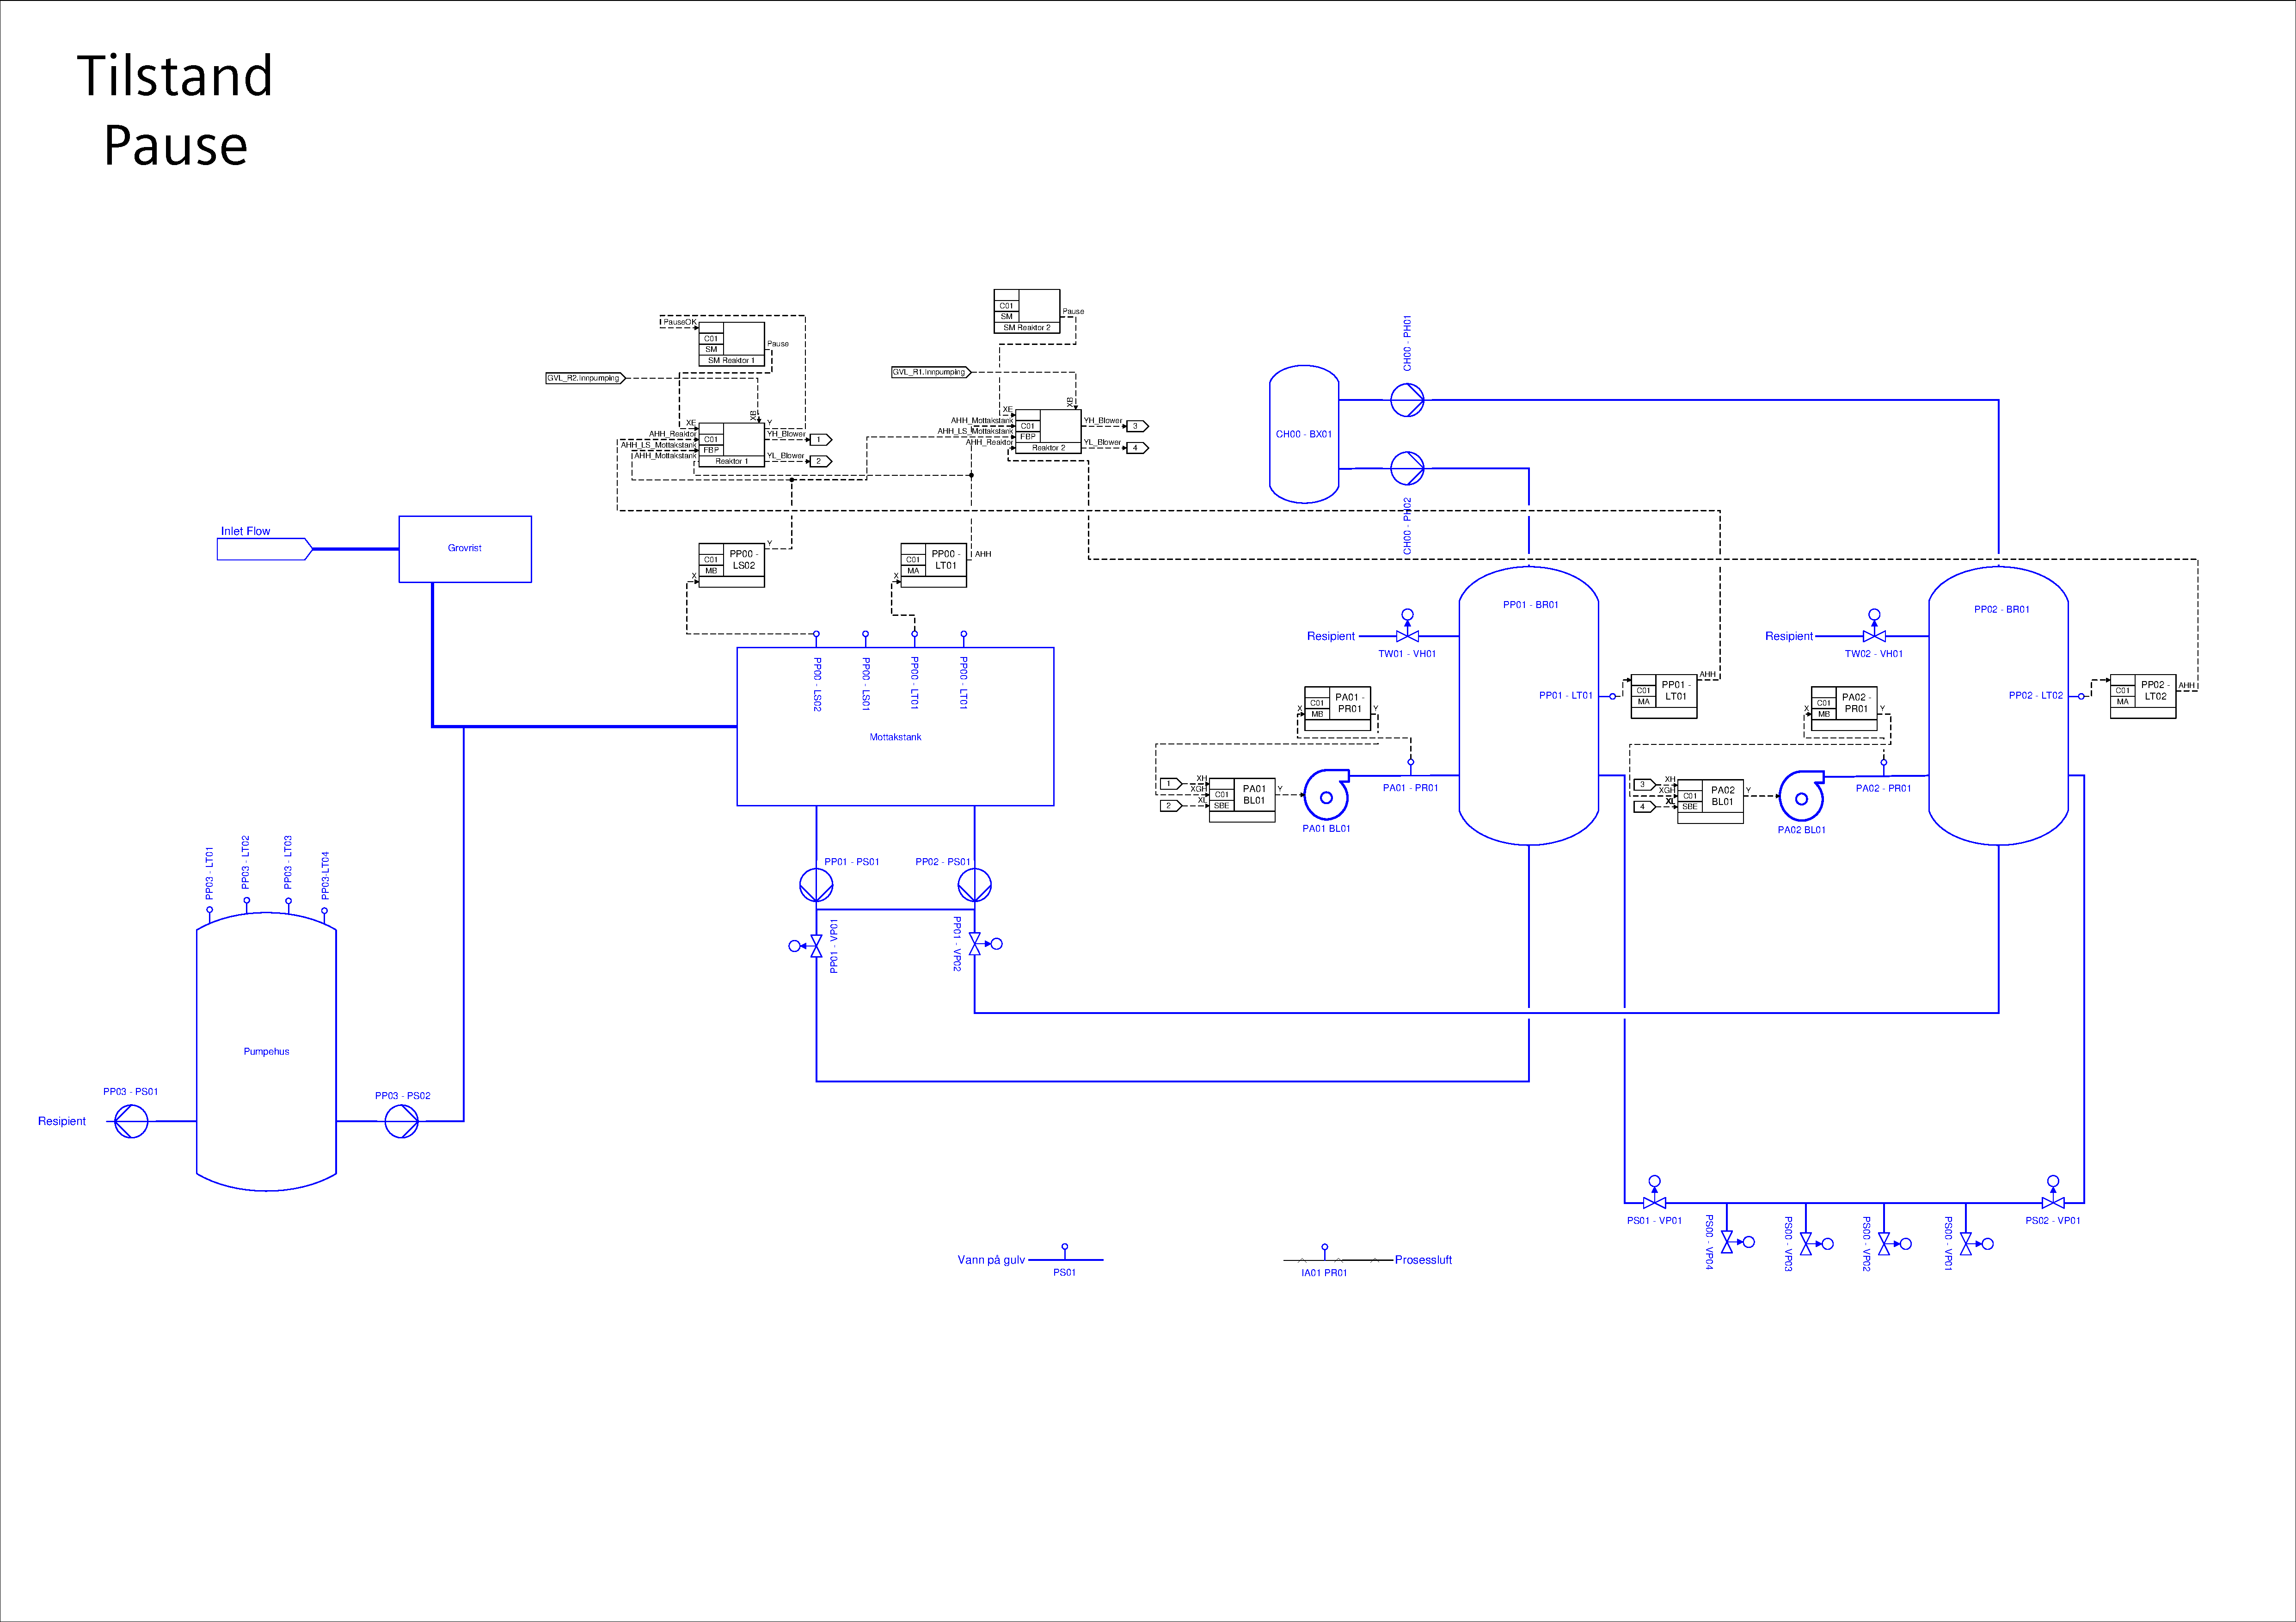
\includegraphics[angle=90, width=\paperwidth, keepaspectratio]{Bilder/SCD.pdf}
    };

    % Place the caption at the bottom of the page
    \node[anchor=south, yshift=10mm] at (current page.south) { % Adjust yshift to position the caption
        \begin{minipage}{\textwidth}
            \centering
            \captionof{figure}{SCD innpumpingssekvens}
            \label{fig:SCD}
        \end{minipage}
    };
\end{tikzpicture

